\documentclass[utf8]{FrontiersinHarvard} % for articles in journals using the Harvard Referencing Style (Author-Date), for Frontiers Reference Styles by Journal: https://zendesk.frontiersin.org/hc/en-us/articles/360017860337-Frontiers-Reference-Styles-by-Journal
%\documentclass[utf8]{FrontiersinVancouver} % for articles in journals using the Vancouver Reference Style (Numbered), for Frontiers Reference Styles by Journal: https://zendesk.frontiersin.org/hc/en-us/articles/360017860337-Frontiers-Reference-Styles-by-Journal
%\documentclass[utf8]{frontiersinFPHY_FAMS} % Vancouver Reference Style (Numbered) for articles in the journals "Frontiers in Physics" and "Frontiers in Applied Mathematics and Statistics" 

%\setcitestyle{square} % for articles in the journals "Frontiers in Physics" and "Frontiers in Applied Mathematics and Statistics" 
\usepackage{url,hyperref,lineno,microtype,subcaption}
\usepackage[onehalfspacing]{setspace}

\linenumbers
\usepackage{minted}

\def\keyFont{\fontsize{8}{11}\helveticabold }
\def\firstAuthorLast{Shumko {et~al.}}
\def\Authors{M. Shumko\,$^{1,2,*}$, D. Chaddock\,$^{3}$, B. Gallardo-Lacourt\,$^{1,4}$, E. Donovan\,$^{3}$, E.L. Spanswick\,$^{3}$, A.J. Halford\,$^{1}$, I. Thompson, and K.R. Murphy}

\def\Address{
    $^{1}$NASA's Goddard Space Flight Center, Greenbelt, Maryland, USA \\
    $^{2}$Department of Astronomy, University of Maryland, College Park, Maryland, USA\\
    $^{3}$University of Calgary in Calgary, Alberta, Canada \\
    $^{4}$Department of Physics, The Catholic University of America, Washington, DC, USA
}
\def\corrAuthor{M. Shumko}

\def\corrEmail{msshumko@gmail.com}

\begin{document}
\onecolumn
\firstpage{1}

\title[AuroraX, PyAuroraX, and aurora-asi-lib]{AuroraX, PyAuroraX, and aurora-asi-lib: a user-friendly auroral all-sky imager analysis framework} 

\author[\firstAuthorLast ]{\Authors} %This field will be automatically populated
\address{} %This field will be automatically populated
\correspondance{} %This field will be automatically populated

\extraAuth{}


\maketitle

\begin{abstract}
\section{}
Within the context of the Heliophysics Observatory, optical images of the aurora are emerging as an important resource for exploring multi-scale geospace processes. This capability has never been more important as we are on the cusp of a new era of geospace research, by which we mean studying the overall system as a ``system of systems". Historically, the patchwork of ground-based instrumentation has required customized solutions for accessing data, assessing data relevance, and then ultimately using each individual network alongside other assets. Here we present a new approach for data discovery and utilization for one ground-based instrument type, the all-sky imager (ASI). The AuroraX project (\url{https://aurorax.space/}) is a comprehensive platform for the discovery of and access to optical auroral data. In this paper, we discuss the AuroraX platform and its API and web-based tools; PyAuroraX, a Python library that can programmatically interface with the AuroraX platform; and aurora-asi-lib, a Python library for interacting with and analyzing high-resolution auroral data. Together, these tools enable a rapid and streamlined end-to-end exploration of auroral data. We demonstate this with an example conjunction study: we show how AuroraX---or PyAuroraX---identifies conjunctions between ground- and space-based instruments. This conjunction discovery is proceeded by looking at summary data from the available imagers for interesting auroral activity. Lastly, we show how you can use the list of conjunctions, together with aurora-asi-lib, to download, load, and analyze ASI data directly on a personal computer.
\tiny
 \keyFont{ \section{Keywords:} THEMIS, REGO, aurora, precipitation, all-sky-imager, precipitation, python, IDL, keogram, conjunction, ionosphere, magnetosphere}
\end{abstract}

\section{Introduction}\label{intro}
Since the 1960s the space physics community has utilized optical ground-based instrumentation that has led to discoveries from which great advancements in the field have been derived. Some of these discoveries include the early description of a substorm introduced by \citet{Akasofu1964}, and several descriptions of new phenomena that highlight the tight connections between the magnetosphere and ionosphere \cite[e.g.][]{Angelopoulos2008, Jones2013, Shumko2021}. These discoveries were possible with a multitude of instruments. 

Meridian Scanning photometers (MSPs), such as the Canadian Auroral Network for the OPEN (Origins of Plasmas in Earth's Neighborhood) Program Unified Study (CANOPUS) array, were first utilized for remote sensing the high-latitude ionosphere \citep[e.g.][]{Rostoker1995}. These one-dimensional MSPs were later followed by two-dimensional All-sky Imagers (ASIs) that took the space physics field into a deeper understanding of the coupled ionosphere-magnetosphere system. In the present day, the space physics community has carried a long legacy of ground-based optical instruments, including the large array from the Time History of Events and Macroscale Interactions during Substorms (THEMIS) ASI observatories \citep{Donovan2006, Mende2009}. Currently, many different optical arrays are in operation or are in development including THEMIS, REGO, MANGO, TREx, and PWING  \citep[e.g.][]{Liang2016, Shiokawa2017, Lyons2019, Gillies2019} \textcolor{red}{Bea: add the MANGO Citation. Hint: asti bath}. These modern ASIs work continuously in high temporal and spatial resolution: each camera producing thousands of images per night.

The rapidly increasing volume of imager data, together with unique data formats, significantly burdens space physicists with mundane and duplicated software engineering tasks---download data, load and correctly parse the data, etc. This unnecessary burden can lead to mistakes in the analysis software that may require unnecessary troubleshooting time from the ASI team, or more worrisome---lead to inaccurate and misleading findings getting published. Thus, robust auroral analysis tools are required.

We introduce the AuroraX project which aims to overcome the above issues by providing key tools to aid auroral researchers. The first tool is the AuroraX website and Virtual Observatory. This website provides various interfaces for quickly visualizing summary data (i.e. keograms, movies, etc.), determining what imagers operated at a given time, and search for conjunctions between numerous ground- and space-based instruments. The second tool is PyAuroraX, a Python library to programmatically interact with the AuroraX platform. The third tool is aurora-asi-lib, a Python all-sky imager library that provides functions to download, load, analyze, and visualize THEMIS and REGO ASI data on a personal computer. 

\section{AuroraX}\label{aurorax}
The motivating driver of the development of the AuroraX cyberinfrastructure project is to enable data mining and analysis of existing and future auroral data with a set of tools specifically designed for exploring auroral observations. With these tools the project would enable key science discovery and enhance the benefits of the world's auroral instrumentation. This is being accomplished with the development of key systems/standards for uniform metadata generation and search, image content analysis, interfaces to leading international tools, and a community involvement that includes more than 80\% of the world's data providers. 

The AuroraX website, located at \url{https://aurorax.space}, is designed to be the first place to start your auroral analysis. The website currently provides interfaces for: performing conjunction searches, exploring summary data such as keograms and movies, viewing information about what data is in the platform (data availability), and documentation about the platform including guides for using the API and client libraries (eg. PyAuroraX).

\subsection{Data Repository}
Fundamentally AuroraX processes a rich database of metadata, which we refer to as the \textit{data repository}. Indeed, AuroraX does not contain any raw data, only metadata and various summary data products. Our goal with this approach is to ease any concerns with data ownership and stewardship that may cause hesitancy to have their data publicly available and searchable by AuroraX. In other words, AuroraX is meant to be a centralized data exploration and event discovery platform and not a raw data repository. This architecture keeps the data repository slim and optimized for the search engine.

The metadata in the AuroraX data repository is currently organized into two categories: 
\begin{itemize}
    \item \textit{ephemeris} records which provide location and operational information for a given ground- or space-based instrument, and
    \item \textit{data product} records describing keograms or other summary products (no images are stored in the database, only URLs which are used as unique identifiers).
\end{itemize} \textit{Ephemeris} data are 1-minute location records when a ground-based or space-based instrument collected data. This allows applications such as the search engine to return more useful query results---ones where there definitively exists raw data that can be further evaluated by auroral researchers. On the other hand, the \textit{data product} consists of records describing summary data in the form of, for example, keograms and timelapse movies. These records are accessed via a unique website URL where the data product lives, allowing this data to be served by each organization that produces ASI data.

Both \textit{ephemeris} and \textit{data product} records can contain any number of arbitrary metadata fields (metadata about metadata) which can be used by the search engine to assist with further levels of filtering and data discovery.

\subsection{Search Engine}
The THEMIS ASI array has generated more than 100 terabytes of data since becoming operational in 2005, with the instruments continuing to generate new data every day. In addition, other ASI arrays such as REGO and TREx produce a combined $>100$ terabytes per year. Sifting through such a large data volume for isolated times with scientific importance is time consuming for the best of auroral scientists. This process of ``event discovery" can be simplified and streamlined by leveraging a database of metadata describing auroral data and its optical content. By combining AuroraX’s aforementioned \textit{data repository} with a search algorithm, we are able to provide scientists with a way to significantly reduce the amount of time spent searching through these datasets for auroral events. 

One AuroraX search engine function is the Conjunction Search. It is designed to quickly provide scientists with periods of time for which two or more ground- or space-based instruments were operating, and were magnetically conjugate. A conjunction search engine with the ability to filter by ASI metadata is the key differentiating factor of AuroraX. As a platform that is built specifically for auroral data, we tailored the search algorithm to consider pertinent information about the instruments and build tools focused on maximizing their scientific contributions. This is in contrast to other conjunction search tools, such as Satellite Situation Center (SSCWeb), that are missing important metadata about the instrumentation that are vital to determining if the conjunction is of importance (ie. instrument collected data or not, operating mode, certain type of aurora was visible or not, etc.).

Conjunction searches can be performed using the AuroraX Conjunction Search webpage (\url{https://aurorax.space/conjunctionSearch/standard}), the AuroraX API, or client libraries like PyAuroraX and IDL-AuroraX (for the Python and IDL programming languages, respectively). The web interface provides several elements to customize a conjunction search using a series of dropdown menus and filter boxes. These include specifying the start and end time, ground instruments and/or spacecraft to find conjunctions between, maximum distance between the instruments (kilometers between magnetic footprints), and conjunction type. Searches can be further refined by using a customizable set of filters on the metadata in the AuroraX Data Repository. These filters are very flexible and easy to adjust for each ASI array or spacecraft instrument. Some examples include instrument operating mode, quality flags, and predicted auroral image content based on machine learning models. One example search is for find all conjunctions between any THEMIS or TREx ASIs with any THEMIS spacecraft, when the spacecraft was in the plasma sheet.

\subsection{Virtual Observatory}
\textcolor{red}{Eric – maybe a paragraph of text talking about previous VOs and the experience over the years of building these}

The AuroraX Virtual Observatory is working towards providing interactive visualizations and data browsing interfaces to quickly navigate the vast amount of auroral data available in the platform. These interfaces are designed to allow a user to browse through the \textit{data repository} in a simple and efficient manner. AuroraX currently has two components to the Virtual Observatory: Keogramist, and the Event Explorer.

As the name implies, the Keogramist (\url{https://aurorax.space/keogramist}) visualizes keograms---a highly compressed summary product for quickly analyzing ASI data. It is a compression of sequential ASI images into a single image that shows pixel intensity as a function of latitude and time. Typically, they are assembled by looping over every image and taking a vertical slice through the center of the image (or through a custom path such a path of a satellite). Objects in the sky such as auroral arcs, pulsating aurora, substorms, clouds, the moon, etc. have unique keogram signatures that allow for a quick interpretation. Keogramist presents keograms from any number of ASI instruments in the AuroraX data repository in a compact and visually-appealing interface. Figure \ref{fig1}(A) shows an example of the TREx keograms from 21 March 2020. When a user identifies a day of interesting auroral activity, they can quickly view additional summary data such as timelapse movies. Keogramist also allows you to filter the keograms displayed based on the data product record metadata fields in the data repository. This could be as simple as the green-channel content in an RGB-based ASI, or more complex such as classifications derived from a machine learning model (ie. pulsating aurora in the field-of-view).

\begin{figure}
    \centering
    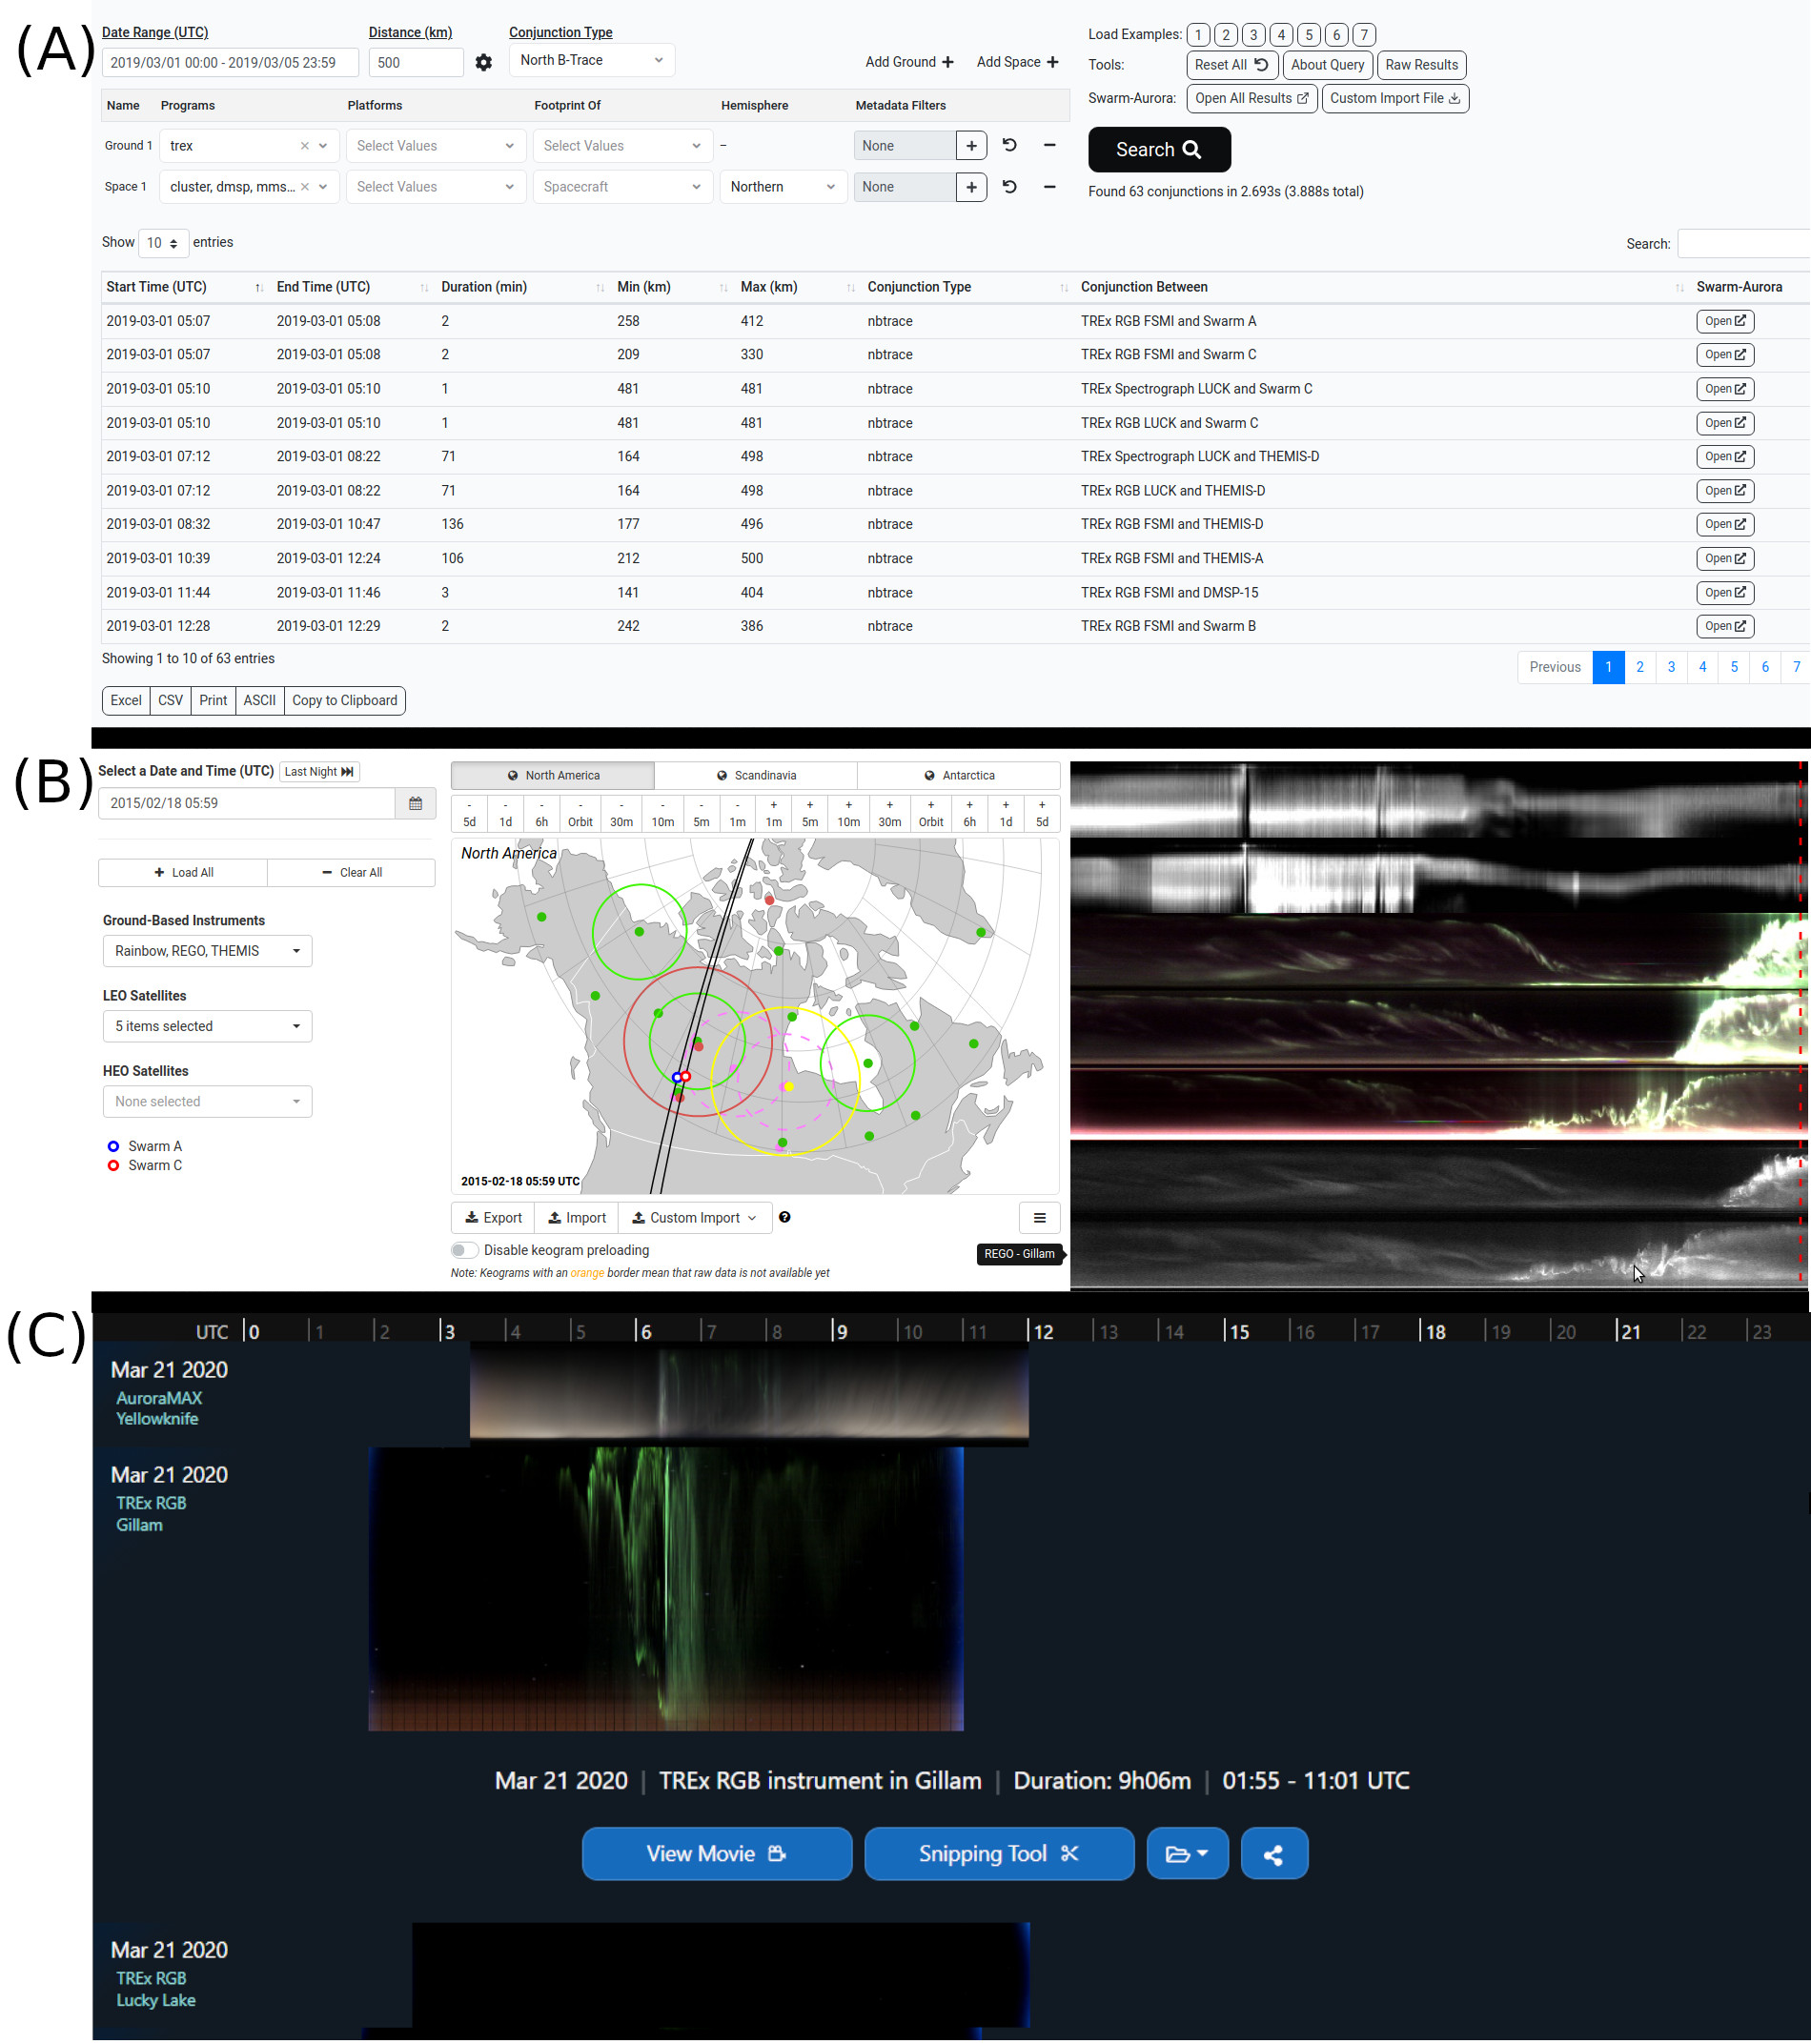
\includegraphics[width=0.9\textwidth]{figures/fig1.jpg}
    \caption{The \url{https://aurorax.space/} website. Panel (A) shows the Keogramist for three TREx ASIs on 21 March 2020. The Gillam keogram is expanded to show further options. Panel (B) shows the conjunction finder with keograms. And lastly, panel (C) shows the conjunctions in list form.}
    \label{fig1}
\end{figure}

The Event Explorer (\url{https://aurorax.space/eventExplorer}) is a 3D visualization of AuroraX ephemeris data with ground-based auroral images projected onto an interactive globe. This tool is designed to assist with visualizing auroral data and evaluating possible conjunctions using a more interactive and global interface. The auroral images are mapped to a 1024x512 grid covering $-180^\circ$ to $180^\circ$ degrees in longitude, and $-90^\circ$ to $90^\circ$ latitude ($0.33^\circ$ and $0.35^\circ$ longitude and latitude resolution), and visualized onto the globe. The grid format was first developed by NOAA and used as part of their 30-min auroral prediction OVATION model outputs. AuroraX has adopted this grid format to provide a global view of summary ASI data alongside representations of spacecraft geographic positions and magnetic footprints, provided by SSCWeb.

In addition to the Keogramist and the Event Explorer, the continued development of the Swarm-Aurora website has become a part of AuroraX’s priorities (\url{https://swarm-aurora.com}). One recent improvement has been the integration of AuroraX with Swarm-Aurora, allowing users to browse Swarm-Aurora using the AuroraX Conjunction Search results. To demonstrate this, Fig. \ref{fig1}(B) shows an example of a conjunction search query, and Fig. \ref{fig1}(C) shows a detailed view of one conjunction. Lastly, architectural design changes were made to Swarm-Aurora to enhance the experience for users around the world, specifically optimizing loading times. Swarm-Aurora now operates on commercial cloud infrastructure in four regions; one in Calgary, two in the United States, and one in Europe. Adding more regions is trivial and can be done as the user base grows and are needed.

\subsection{PyAuroraX}
An important part of any platform like AuroraX is to allow users to leverage the data for use in their own scientific analyses and applications. To assist with these tasks, we developed software to interact with AuroraX using only a few lines of code. This is enabled by the AuroraX API and subsequent client libraries maintained by the project, one of which is PyAuroraX (\url{https://github.com/aurorax-space/pyaurorax}).

PyAuroraX allows users to interact with the AuroraX API and perform \textit{conjunction}, \textit{ephemeris}, and \textit{data product} searches using Python. For example, the \verb|pyaurorax.conjunctions.search()| function can be used to search AuroraX for conjunctions in the same way the AuroraX Conjunction Search webpage allows (\url{https://aurorax.space/conjunctionSearch/standard}). The below Python code shows how to perform a simple search, asking AuroraX to find all conjunctions between several instruments from the THEMIS ASI array and any Swarm spacecraft.

\begin{minted}{python}
import pyaurorax
import datetime

# define search parameters
start = datetime.datetime(2019, 1, 1, 0, 0, 0)
end = datetime.datetime(2019, 1, 3, 23, 59, 59)
ground_params = [
    {
        "programs": ["themis-asi"],
        "platforms": ["fort smith", "gillam"],
    }
]
space_params = [
    {
        "programs": ["swarm"],
        "hemisphere": ["northern"],
    }
]
distance = 500

# perform conjunction search
s = pyaurorax.conjunctions.search(start=start,
                                  end=end,
                                  distance=distance,
                                  ground=ground_params,
                                  space=space_params,
                                  verbose=True)
\end{minted}

Users can also retrieve other information from AuroraX such as data sources, \textit{ephemeris} records, \textit{data product} records, and data availability. All functions in PyAuroraX are also available for use with IDL programs by using the IDL-AuroraX library (\url{https://github.com/aurorax-space/idl-aurorax}). 

Documentation and examples are a key part of helping new users learn what is possible and provides a reference for more experienced users. To assist with this and ease the learning curve, AuroraX has developed a documentation website, available at \url{https://docs.aurorax.space}, with technical details about the platform, the metadata in it, and the various applications and tools available for use. Extensive examples and code snippets are available in the ``Developer Zone" to provide quick and simple uses of key programmatic tasks. The source code for this website is also available on Github alongside other open-source codebases within the AuroraX project (\url{https://github.com/aurorax-space/docs}). 

\section{Analyzing high-resolution ASI data using aurora-asi-lib}\label{aurora-asi-lib}
The final component of AuroraX is aurora-asi-lib, henceforth referred to, and imported as, asilib. It enables researchers to apply common data analysis tasks to the THEMIS and REGO ASI image data on a personal computer. Here we overview the main functions, while the online documentation at \url{https://aurora-asi-lib.readthedocs.io/} contains more examples, a tutorial, and a thorough API reference.

As we tour a few asilib functions, keep in mind that asilib is designed to manage the lower-level tasks. For example, if you want to load the image data via \verb|asilib.load_image()|, asilib will attempt to download the 1-hour Common Data Format (CDF) data if it is not already saved on your computer. Likewise, if you call \verb|asilib.plot_keogram()|, it will automatically load (and download if necessary) the ASI data before plotting it. For reference, Figs. \ref{fig2}-\ref{fig4} were made using the code in a Jupyter Notebook that is provided as supplemental material in both the ipynb and pdf formats.

\subsection{Plotting single images}
One common way to visualize all-sky images is with \verb|asilib.plot_fisheye()|. It plots the raw ASI images oriented with North at the top and East to the right of each image. The term fisheye comes from the fisheye lens that expands the imager's field of view to nearly $180^\circ$. Figure \ref{fig2}(A and C) show an example of an auroral arc observed concurrently by the THEMIS and REGO ASIs stationed at Rankin Inlet (RANK). By default the color map is automatically chosen: black-to-white for THEMIS and black-to-red for REGO. The default color scale is dynamically calculated using percentile logic described in the documentation.

The other common way to visualize images is by projecting the fisheye image onto a geographic map using \verb|asilib.plot_map()|. asilib uses the skymap files to map each pixel's vertices to a (latitude, longitude) point at an aurora emission altitude, typically assumed 110 km for THEMIS and 230 km for REGO \citep{Donovan2006, Liang2016}. Figure \ref{fig2}(B and D) show the fisheye images mapped to 110 km altitude. By default, pixels that look at elevation $< 10^\circ$ are not mapped due to nearby obstructions and the stretching of pixels closest to the horizon. And lastly, \verb|asilib.make_map()| provides a default geographic map to project the images onto.

\begin{figure}
      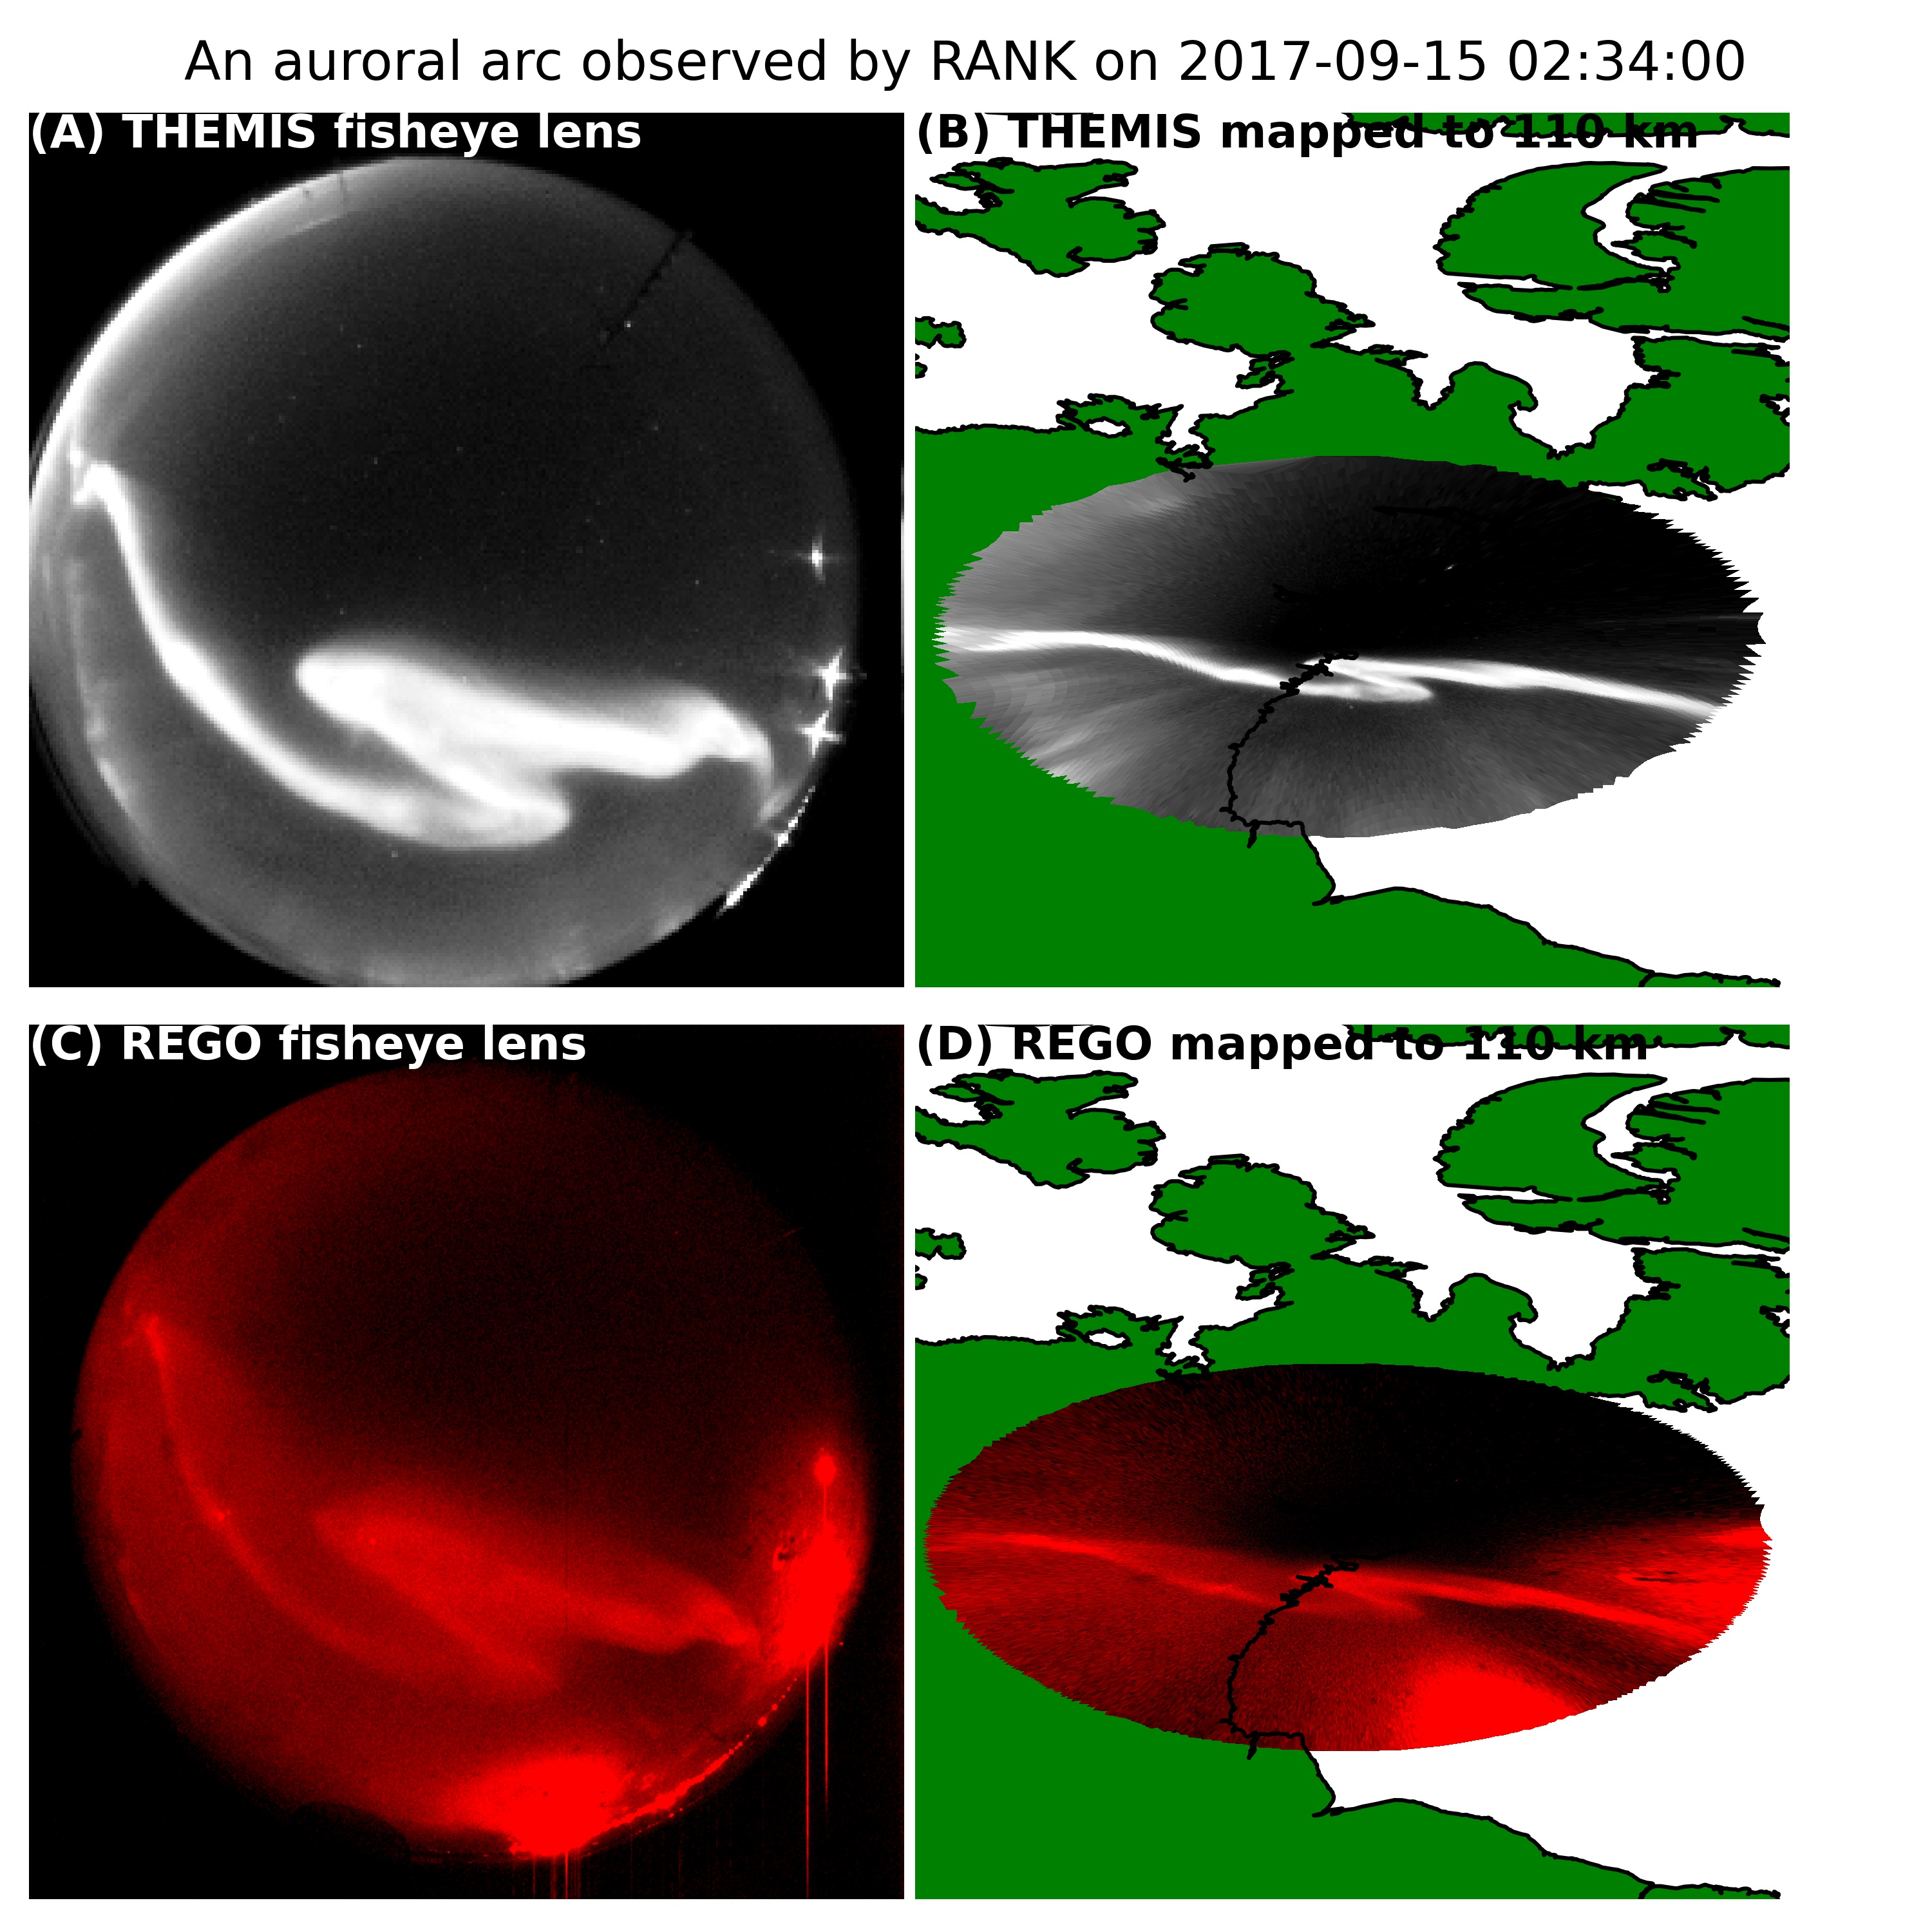
\includegraphics[width=\textwidth]{figures/fig2.jpg}
      \caption{An auroral arc observed simultaneously by the REGO and THEMIS imagers at Rankin Inlet, Canada. Panels (A) and (C) show the fisheye lens view, while panels (B) and (D) show the same images projected to the 110 km assumed aurora emission altitude. Only the pixels with elevation $>10^\circ$ are plotted.}
      \label{fig2}
\end{figure}

\subsection{Keograms}
You can make a keogram using the \verb|asilib.plot_keogram()| function that takes an optional \verb|map_alt| keyword argument. If it is not provided, the keogram's vertical axis is pixel index, as we show in Fig. \ref{fig3}(A). If a valid map altitude is provided, the vertical axis is geographic latitude as we show in Fig. \ref{fig3}(B). Lastly, by providing \verb|map_alt| and setting \verb|aacgm=True|, the vertical axis becomes magnetic latitude in the Altitude-adjusted corrected geomagnetic coordinate system (AACGM) \citep{Shepherd2014}.
The latitude transformation between Fig. \ref{fig3}(A) and Fig. \ref{fig3}(B) is substantial---the low elevation pixels observe much wider regions of latitude, compared to the pixels at higher elevations.

\begin{figure}
      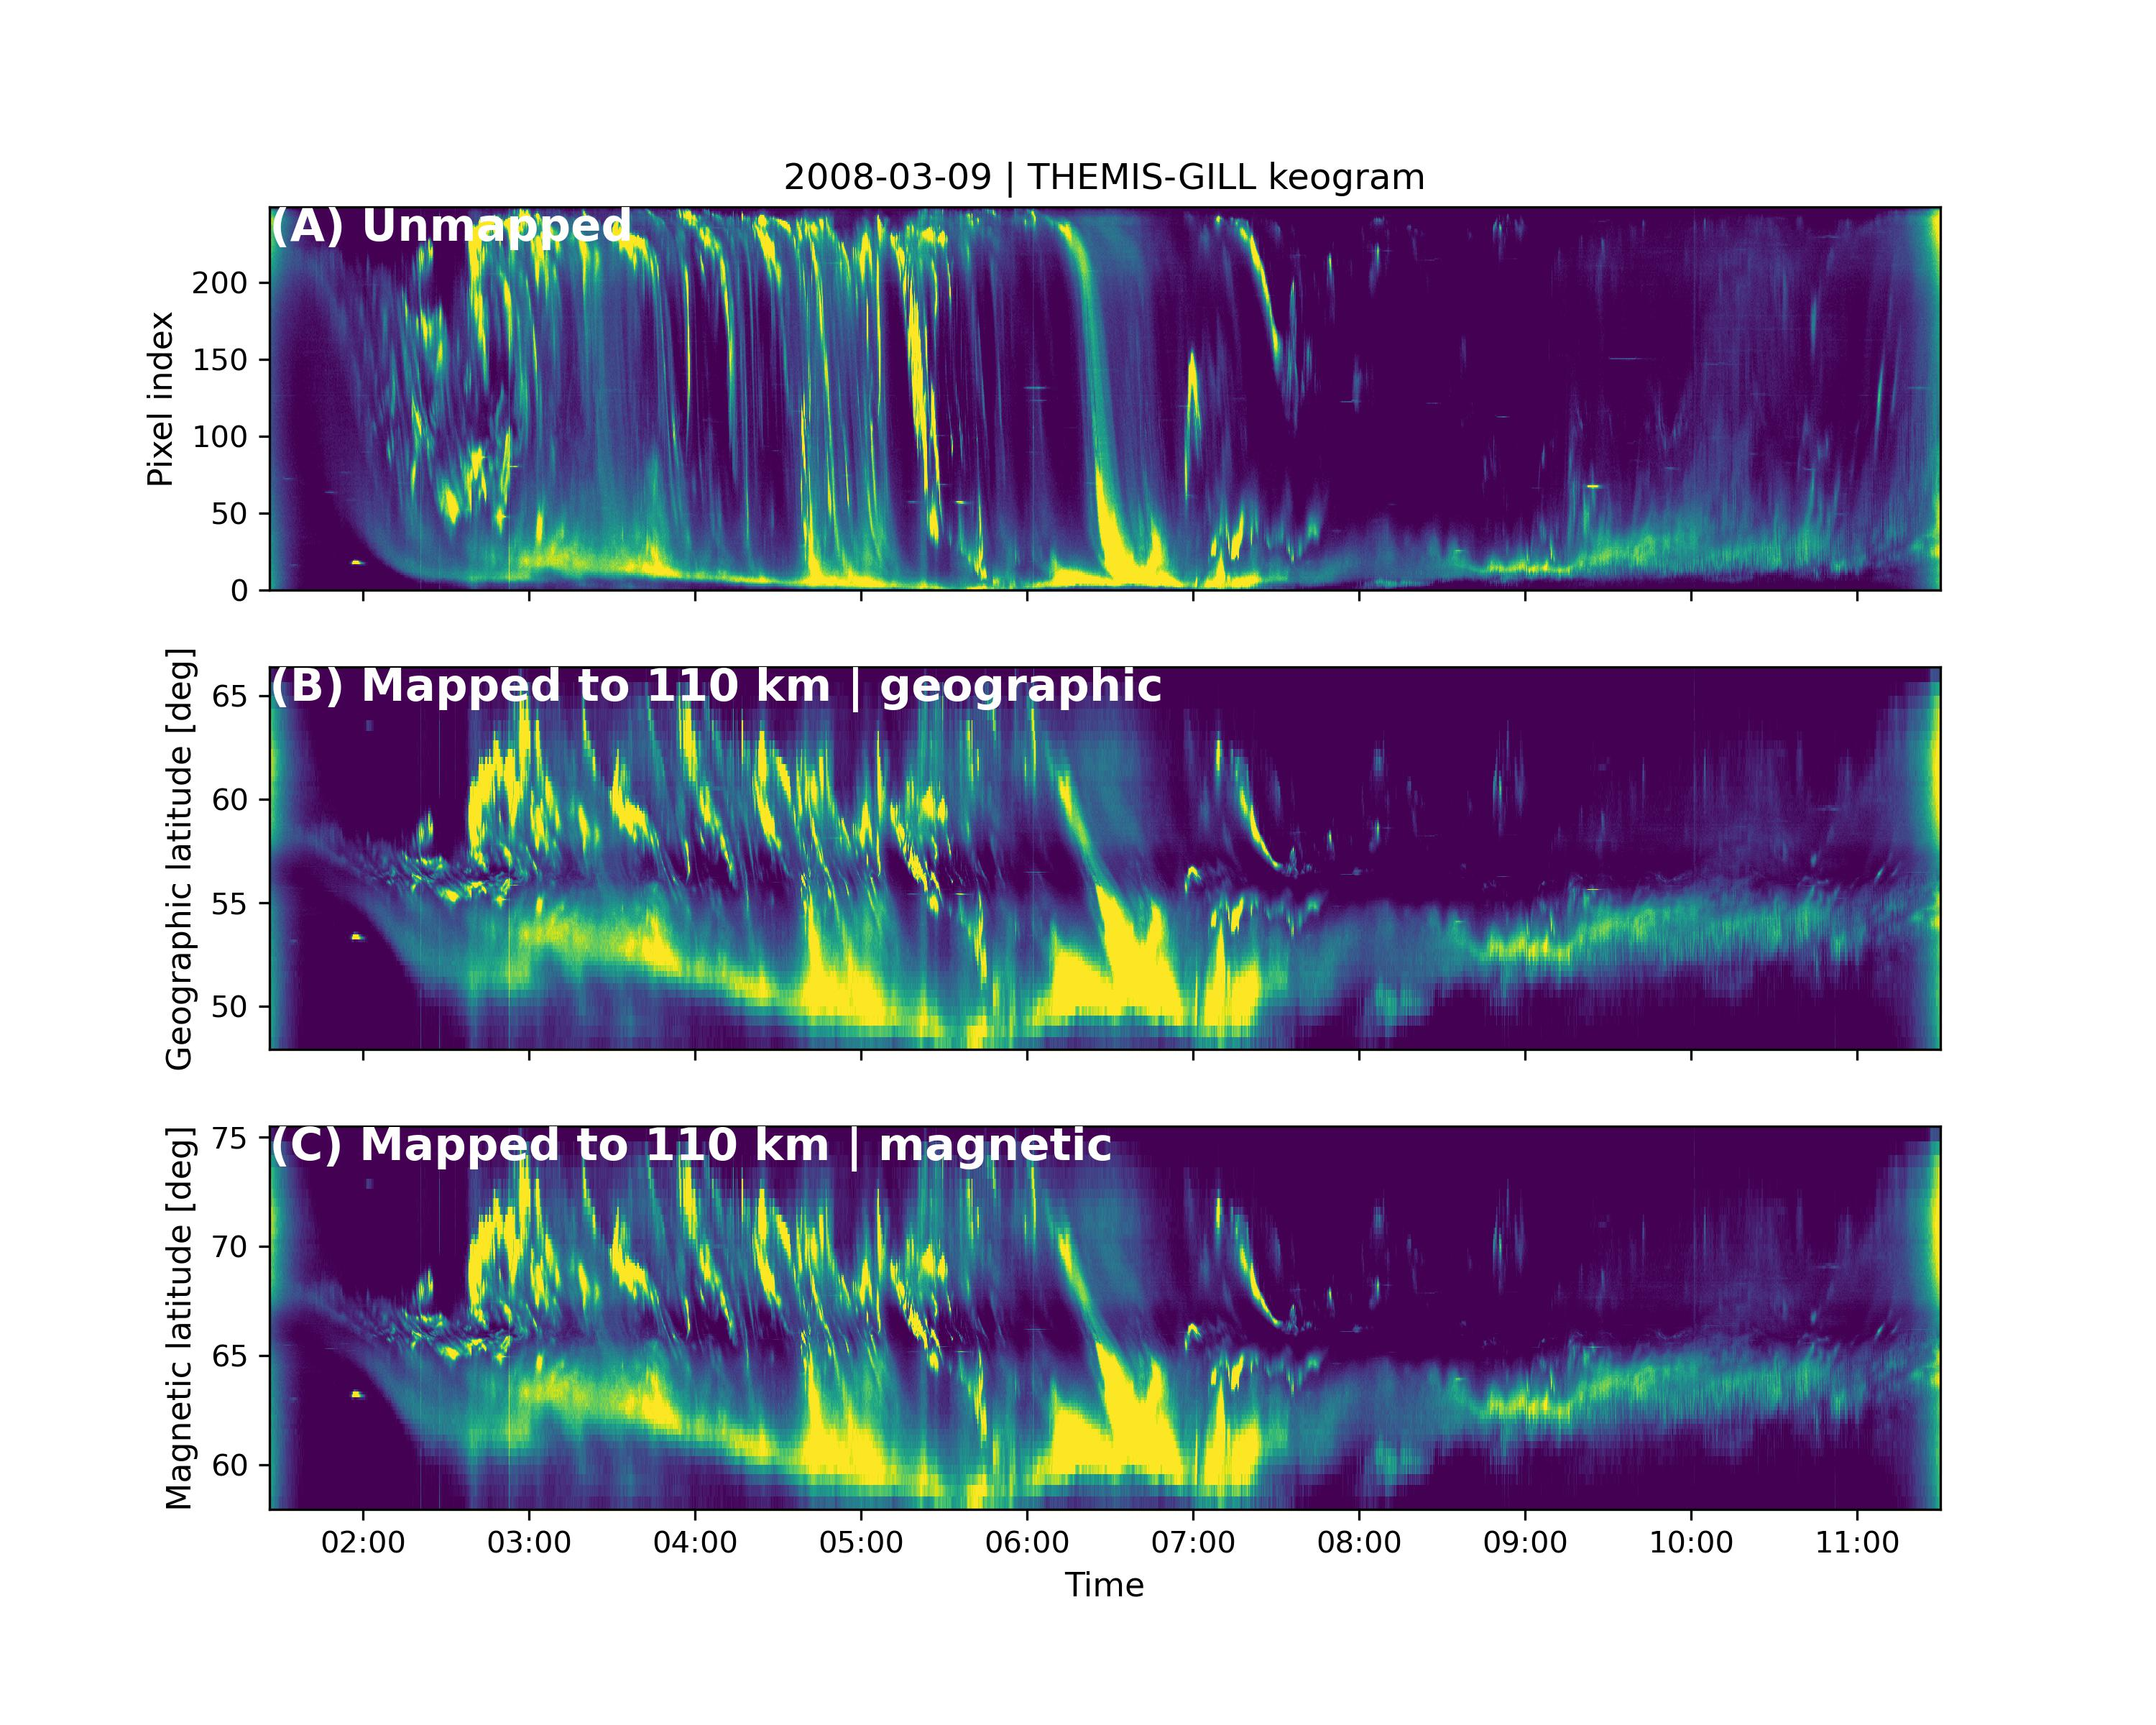
\includegraphics[width=\textwidth]{figures/fig3.jpg}
      \caption{A full-night keogram showing the dynamic aurora observed at Gillam, Canada on 9 March 2008. Panel (A) shows the unmapped keogram with the pixel index vertical axis, panel (B) shows the geographic latitude of the pixels mapped to 110 km altitude. Lastly, panel (C) shows the corresponding magnetic latitudes.}
      \label{fig3}
\end{figure}


\subsection{Animating Images}
asilib allows you to easily animate the ASI fisheye and mapped images using \verb|asilib.animate_fisheye()| and \verb|asilib.animate_map()|. It first saves png images in a \\ \verb|asilib.config['ASI_DATA_DIR']/animations/images/| folder, and then animates them using the \verb|ffmpeg| library \citep{ffmpeg} . Animation S1 in the supporting document shows an example animation of auroral streamers.

Animating just the images is somewhat limiting. Thus, \verb|asilib| also includes \\ \verb|asilib.animate_fisheye_generator()| and \verb|asilib.animate_map_generator()| (which are technically coroutines) to modify the animations as they are made. This is useful, for example, if you need to draw the satellite's location in each image.

\subsection{Conjunction analysis tools}
Currently, \verb|asilib| provides three functions that are useful for analyzing conjunctions: \verb|asilib.lla2footprint()|, \verb|asilib.lla2azel()|, and \verb|asilib.equal_area()|.

\verb|asilib.lla2footprint()| uses IRBEM-Lib (\citet{irbem}; requires a separate installation and compilation of the Fortran source code) to trace a satellite's position, in geographic (latitude, longitude, altitude) (LLA) coordinates, along a magnetic field line. This field line is defined using one of the magnetic field models that are supported by IRBEM. The primary use of this function is to map a satellite's location from, for example, 500 km altitude, to its magnetic footprint at the assumed auroral emission altitude (e.g. 110 km for THEMIS or 230 km for REGO as previously mentioned).

The next function is \verb|asilib.lla2azel()|. This function maps the satellite's footprint location, in LLA coordinates, to the ASI's (azimuth, elevation) coordinates (AzEl) using the skymap files. This function returns both the AzEl coordinates as well as the corresponding pixel indices.

Lastly, \verb|asilib.equal_area()| calculates a mask of pixels inside an auroral emission area---useful to calculate the mean ASI intensity (or another statistical quantity) in a physical area in the sky. The mask contains 1s inside of the area and \verb|numpy.nan| outside of it. You then multiply the image with the mask: the pixel intensities outside of the area are then \verb|numpy.nan| and unchanged inside the area. We chose to use \verb|numpy.nan| to ensure that the mean of the intensity is correctly applied---it will fail if you call \verb|numpy.mean(image*mask)|, but \verb|numpy.nanmean(image*mask)| will ignore NaNs and correctly calculate the mean intensity inside the area.

\subsection{Analyzing a conjunction}\label{satellite_conjunction}
In this example we combine the aforementioned analysis functions to calculate the mean auroral intensity surrounding the footprint of an artificial satellite during a conjunction with a THEMIS ASI. This satellite orbits at a 500-km altitude low Earth orbit. We will first calculate the mean ASI intensity in a 20x20 km area at a 110 km altitude and then animate the conjunction. Using an artificial satellite allows us to clearly exemplify how any satellite's footprint could be easily added by using the aurora-asi-lib tool. 

For this example we use the satellite's location in LLA coordinates with time stamps that line up with the ASI times. In reality, the satellite and ASI time stamps are unlikely to line up, so you'll need to align the satellite's and ASI's time stamps.

Our analysis consists of three main steps:
\begin{enumerate}
    \item Trace the satellite's position along the magnetic field line to 110 km using  \verb|asilib.lla2footprint()|.
    \item Locate the satellite's footprint in the imager's field of view (azimuth and elevation coodinates) using \verb|asilib.lla2azel()|.
    \item Calculate the auroral intensity surrounding the satellite's footprint. We create a 20x20 km area mask using \verb|asilib.equal_area()| and use it to calculate the mean ASI intensity as a function of time (and satellite position).
\end{enumerate} These steps are implemented in the ``Figure 4" section of the \verb|asilib_figures| notebook.

Animation S2 shows the result of this conjunction analysis and Fig. \ref{fig4} shows a five-frame montage summarizing the animation. Fig. \ref{fig4}(A-D) show the fisheye lens images at the annotated time stamps. The satellite's footprint path is represented by the red line and the instantaneous footprint by the red dot. The yellow areas show the 20x20 km area around the footprint. And lastly, Fig. \ref{fig4}(E) shows the mean ASI intensity time series---clearly showing the auroral arc intensity between 2:33:30 and 2:34:15.

\begin{figure}
      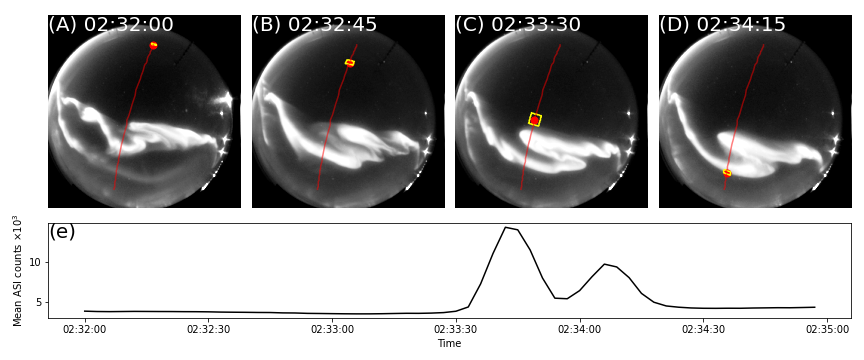
\includegraphics[width=\textwidth]{figures/fig4.png}
      \caption{A conjunction montage of Animation S2. Panels (A)-(D) shows the auroral arc evolution and the satellite's location. The red line is the satellite track and the red dot is its instantaneous position. The yellow quadrilateral bounds the pixels inside the a 20x20 km area surrounding the satellite's 110 km altitude footprint. Lastly, panel (E) shows the mean ASI intensity, as a function of time, inside the yellow quadrilaterals. When the satellite passed through the arc between 2:33:30 and 2:34:15, the mean ASI show two corresponding intensity enhancements.}
      \label{fig4}
\end{figure}

\section{Quality Assurance}
We developed AuroraX, PyAuoraX, and aurora-asi-lib with usability, reliability, and maintainability at the forefront. Documentation is critically important to the survival and usability of software. The AuroraX documentation is hosted at \url{https://docs.aurorax.space/} and the asilib documentation at \url{https://aurora-asi-lib.readthedocs.io/}. There you will find installation instructions, examples, comprehensive tutorials, and API references.

The source code for AuroraX, PyAuroraX, and asilib  is open source and hosted on GitHub. The two Python libraries are also cataloged on Zenodo and can be installed from the Python Packaging Index (PyPI; install using the “pip” command). On GitHub you can submit an Issue for bugs or feature requests, and contribute with a Pull Request.  

To ensure code stability, the codebases for both Python libraries include tests suites that you can run locally and are automatically executed using GitHub Actions every time a change is pushed to the repository. These comprehensive tests check and warn of any software bugs or changes in function behaviour over the course of further development and maintenance.


\section{Conclusion}
The AuroraX website, PyAuroraX, and aurora-asi-lib tools provide the auroral science community with a simple and robust set of analysis tools to enable system-level auroral science. As we demonstrated, these tools provide an end-to-end analysis solution for using auroral data. We described one such solution: to identify and analyze conjunctions. We showed how you can use the AuroraX Conjunction Search website or PyAuroraX to identify and filter conjunctions between a number of ASIs and spacecraft. We then use aurora-asi-lib to quantify the auroral intensity at the satellite's footprint during a conjunction. This example is just one way that AuroraX can help you quickly sift through an immense volume of ASI data to uncover new physics in a significantly less amount of time than was previously possible.

In the near future we will expand AuroraX’s data repository by including more ASI arrays, satellites, and informative metadata filters. Furthermore, TREx and other ASIs will be added to aurora-asi-lib by the current development team and the community. The continued success and usability of AuroraX depends on community contributions. We encourage an open science approach, and look forward to working more broadly within the auroral research community.


\section*{Conflict of Interest Statement}
The authors declare that the research was conducted in the absence of any commercial or financial relationships that could be construed as a potential conflict of interest.

\section*{Author Contributions}
ED, ELS, and DC designed and developed the AuroraX platform and PyAuroraX. AJH, KRM, and IT assisted MS with developing aurora-asi-lib. MS, BGL, DC, and ED wrote the manuscript. ED, ELS, and DC provided the THEMIS and REGO ASI data and expertise.  All authors contributed to manuscript revision, read, and approved the submitted version

\section*{Funding}
MS and BGL acknowledge the support provided by the NASA Postdoctoral Program at the NASA's Goddard Space Flight Center, administered by Oak Ridge Associated Universities under contract with NASA. AJH was supported in part by the Goddard Internal Funding Model which funds the Space Precipitation Impacts team with grant HISFM21. ED, ELS, and DC acknowledge the AuroraX funding sources: the Canadian Foundation for Innovation (CFI), the Province of Alberta, the Technical University of Denmark (DTU, Swarm DISC Program), and the Canadian Space Agency.

\section*{Acknowledgments}
The authors acknowledge all of the scientists, technicians, and engineers who designed, built, and maintain these ASI arrays. The UCalgary team acknowledges the AuroraX, REGO ASI and THEMIS ASI funding agencies and thanks them for their continued support. The UCalgary team also acknowledges the University of Alberta and RPG Consulting for their work on AuroraX. 

\section*{Data Availability Statement}
The datasets and code presented here can be found in the following links.
\begin{itemize}
    \item AuroraX: \url{https://aurorax.space/} and \url{https://github.com/aurorax-space}
    \item AuroraX documentation: \url{https://docs.aurorax.space}
    \item aurora-asi-lib: \url{https://aurora-asi-lib.readthedocs.io/en/latest/}
    \item THEMIS: \url{https://data.phys.ucalgary.ca/sort_by_project/THEMIS/asi/}
    \item REGO: \url{https://data.phys.ucalgary.ca/sort_by_project/GO-Canada/REGO/}
\end{itemize}

\section*{Contribution to the Field Statement}
\noindent The aurora is a ubiquitous light spectacle that has been observed in the polar regions for millennia. The regional scale of the aurora has led to the recent development of numerous all-sky imagers (ASIs)---and arrays of imagers---that continuously take images every night. The large volume of images has quickly become unmanageable by any single group of scientists, leading to datasets that are at best fragmented on the internet, and at worst hidden from the public. The AuroraX project (\url{https://aurorax.space/}) aims to address this problem with a centralized metadata search platform that combines auroral imaging datasets into one easily used resource. This project consists of various tools including a data repository, a search engine, web-based search and analysis interfaces, and software-driven programmatic interfaces (ie. APIs, client libraries such as PyAuroraX). Additionally, the Python library aurora-asi-lib provides the ability to easily analyze high-resolution auroral data from two key ASI arrays – THEMIS and REGO. Together, these tools provide an important improvement to the accessibility and usability of all-sky imager data for auroral science.

\bibliographystyle{Frontiers-Harvard} 
\bibliography{refs}
\end{document}